\documentclass[12pt,fleqn]{article}\usepackage{../../common}
\begin{document}
Eğri Uydurma, Aradeğerleme (Interpolation) - 1

Diyelim ki elimizde alttaki veri var.

\begin{minted}[fontsize=\footnotesize]{python}
x = np.arange(1,7)
y = np.array([10, 5.49, 0.89, -0.14, -1.07, 0.84])
plt.plot(x,y,'.')
plt.ylim(-2,12)
plt.xlim(0,7)
plt.savefig('compscieng_1_21_01.png')
\end{minted}

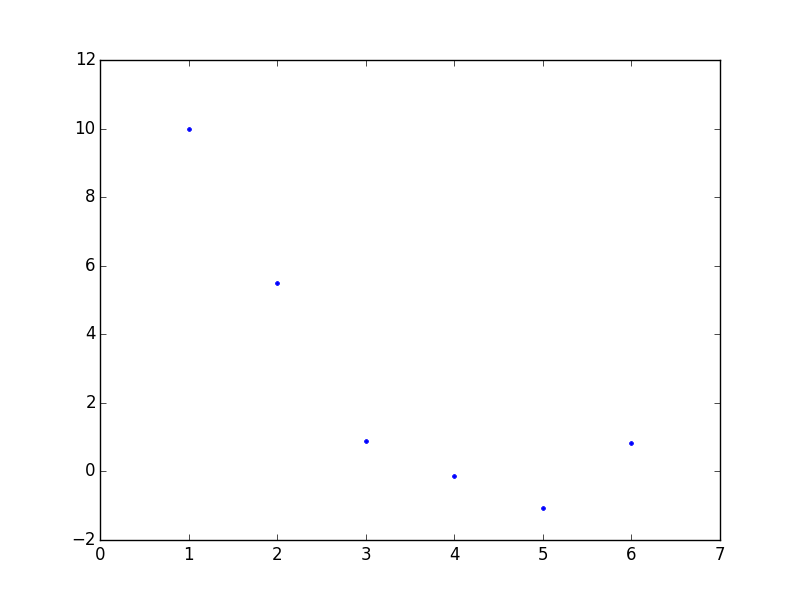
\includegraphics[height=6cm]{compscieng_1_21_01.png}

Bu veriye istediğimiz kadar bükümü olan bir eğri nasıl uydururuz?
``İstediğimiz kadar bükümü olan eğri'' polinom çağrısı yapabilir.. Mesela
bir polinom eğri,

$$ y = c_1 x^3 + c_2x^2 + c_3x + c_4 $$

olarak gösterilebilir. Mesela bazı gelişigüzel sabit değerler
$c_1=1,c_2-20,c_3=1,c_4=-4$ sabitlerinden alttaki görüntü çıkar,

\begin{minted}[fontsize=\footnotesize]{python}
x2 = np.linspace(0,10,1000)
c_1 = 2.; c_2 = -20.; c_3 = 1.; c_4 = -4
y2 = c_1*x**3 + c_2*x**2 + c_3*x + c_4
plt.plot(x2,y2)
plt.savefig('compscieng_1_21_02.png')
\end{minted}

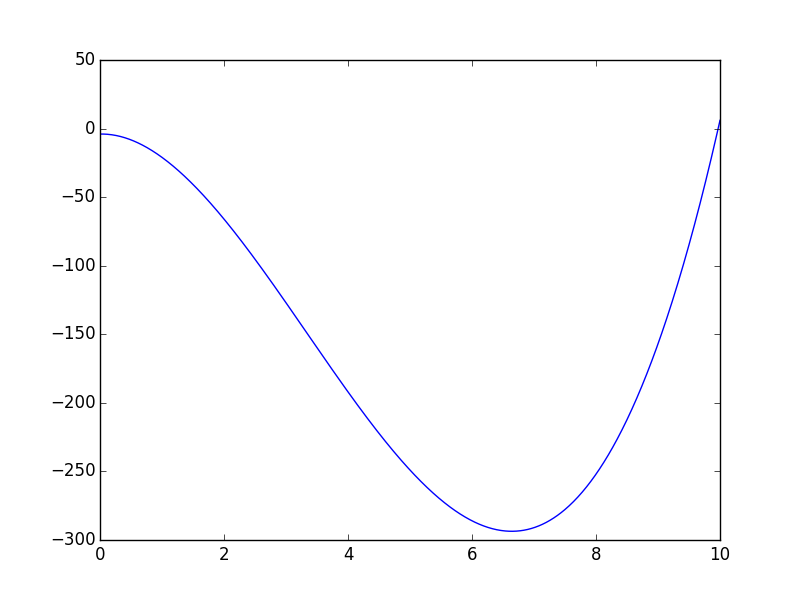
\includegraphics[height=6cm]{compscieng_1_21_02.png}

Eğri iki kere bükülebiliyor çünkü formül küpsel. Karesel olsa sadece bir
kere bükülebilirdi. Peki karesel, ya da küpsel ya da daha üst derecedeki
polinomları veriye nasıl uydururuz? Acaba lineer regresyonu bir şekilde
kullanabilir miyiz? Ama lineer regresyon, adı üstünde, ``lineer'', yani
doğrusal. Doğrusal olmayan bir şeyi nasıl uyduracağız? Şimdi lineer
regresyonun neyi uydurduğunu hatırlayalım,

$$ y = c_1 z_1 + c_2 z_2 + .. + c_nz_n $$

Bu çok boyutlu, her biri birer vektör olan $z_1,..,z_n$ ile tek vektör $y$
ilişkisini girdi olarak alıyor (üstteki formülü ya vektörsel işlem olarak
ya da $y,z_i$ öğelerinin teker teker formüle geçildiği şekilde
görebiliriz). 

Acaba şöyle bir numara yapamaz mıyız? Eğer elimizdeki tek boyutlu veriyi
alıp, onun tamamının bir kere karesini, bir kere küpünü, vs. ayrı ayrı alıp
her sonucu sanki ayrı bir boyutlarmış gibi lineer regresyona verirsek,
otomatik olarak eğri uydurmuş olmaz mıyız ?! Yani üstteki örnek için
$z_1=x^3,z_2=x^2,z_3=x,z_4=1$ olacak, matris formunda,

$$ A = 
\left[\begin{array}{rrrr}
x_1^3 & x_1^2 & x_1 & 1 \\
x_2^3 & x_2^2 & x_2 & 1 \\
\vdots & \vdots & \vdots & \vdots \\
x_m^3 & x_m^2 & x_m & 1 
\end{array}\right]
 $$

ki $x_i$, $x$ vektörünün tek bir öğesini temsil ediyor. Gerisi bildiğimiz En
Az Kareler yöntemi ile $Ax=b$'yi, ya da üstteki notasyona göre $Ac=y$
çözmek, $(A^TA)^{-1}A^Tc$ ile (tabii QR kullanmak daha iyi ama bu basit
örnek için önemli değil). Baştaki örneği çözelim mesela

\begin{minted}[fontsize=\footnotesize]{python}
import scipy.linalg as lin
A = np.array([x**3, x**2, x, np.ones(len(x))]).T
res = np.dot(np.dot(lin.pinv(np.dot(A.T,A)),A.T),y)
print A, '\n\n', res
\end{minted}

\begin{verbatim}
[[   1.    1.    1.    1.]
 [   8.    4.    2.    1.]
 [  27.    9.    3.    1.]
 [  64.   16.    4.    1.]
 [ 125.   25.    5.    1.]
 [ 216.   36.    6.    1.]] 

[  0.03925926   0.42313492  -6.5032672   16.12666667]
\end{verbatim}

Kütüphane çağrısı \verb!polyfit! kullanırsak,

\begin{minted}[fontsize=\footnotesize]{python}
print np.polyfit(x,y,3)
\end{minted}

\begin{verbatim}
[  0.03925926   0.42313492  -6.5032672   16.12666667]
\end{verbatim}

Tıpatıp aynı sonuç çıktı, çünkü büyük bir ihtimalle \verb!polyfit! aynı
tekniği kullanıyor! 

\begin{minted}[fontsize=\footnotesize]{python}
plt.plot(x,y,'.')
plt.ylim(-2,12)
plt.xlim(0,7)
yy = res[0]*x**3 + res[1]*x**2 + res[2]*x + res[3]
plt.plot(x,y,'.')
plt.hold(True)
plt.plot(x,yy)
plt.savefig('compscieng_1_21_03.png')
\end{minted}

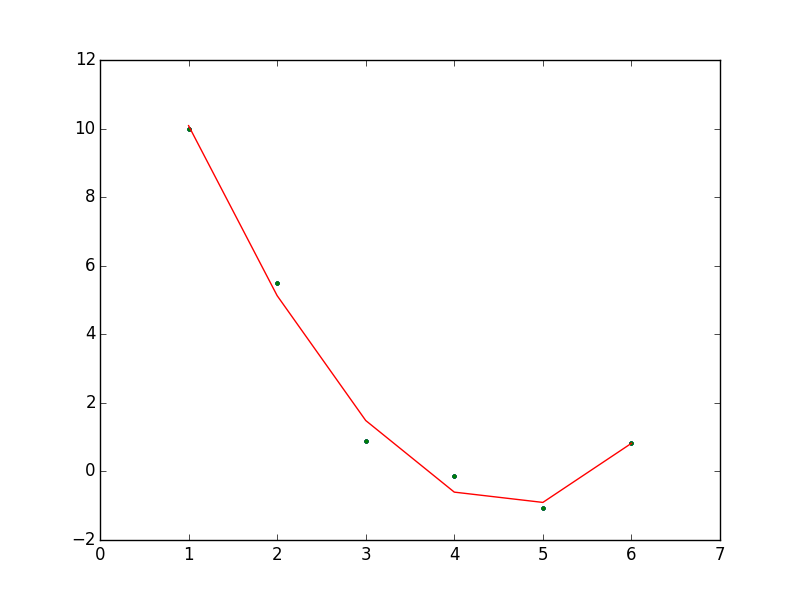
\includegraphics[height=6cm]{compscieng_1_21_03.png}

Uyum fena değil! Not: eğri kesikli çıktı çünkü çok az sayıda veri var. 

Lagrange Aradeğerlemesi (Lagrange Interpolation)

En ekşi ve en yaygın uygulaması olan aradeğerleme fonksiyonlarından biri JL
Lagrange tarafından yayınlanmış olandır. Pratik faydalarının yaninda bu tekniğin
önemli bazı teorik sonuçları var, bu sebeple yaklaşık ya da olmayan entegrasyon
ve türev alma tekniklerini bir fonksiyonu Lagrange aradeğerlemesi ile temsil
etmeyi baz alıyor [1, sf. 268].

Lagrange tekniğinin önemli bir özelliği yaklaşık temsil edilecek fonksiyon için
seçilen değerler üzerinde aynen verinin söylediği değerleri tekrar
üretebilmesi. Yani eğer $f(x)$'i bir $f_h(x)$ ile yaklaşık temsil etmişsek, ve
eğer $f(1) = 3$ ise, aradeğerleme sonrası $f_h(1) = 3$ olacaktır, ve bu
üzerinden aradeğerleme yapılmış tüm veri noktaları için doğru olacaktır.
Ayrıca bu tekniğin önemli bir özelliği üzerinden aradeğerleme yapılan $x$
değerlerinin gelişigüzel seçilebilmesi, eşit aralıkta alınma gibi bir
zorunluluk yok.

Şimdi diyelim ki elde modellenen $f(x)$ için elde $n$ tane $x_1,x_2,...,x_n$
değeri var, ki

$$
f(x_i) = y_i, \qquad i=1,2,..,n
$$

Çözmek istediğimiz problem mümkün olan az derecede olan bir polinom $P_m(x)$
yaratmak öyle ki bu polinom eldeki $(x_i,y_i)$ veri noktalarını temsil
edebilsin, yani

$$
P_m(x_i) = y_i, \qquad i=1,2,..,n
$$

Burada $m$ altsembolü dereceyi göstermek için kullanılıyor.

Daha önce söylediğimiz gibi veri noktalarında aradeğerleme ve veri aynı sonuçta
olmalı.

Bu amaçla $n$ tane ayrı ayrı polinom $p_i(x)$ yaratacağız, ve bu polinomlar
öyle tasarlanacak ki $x_i$ noktasında biri aktif olacak, diğerleri yokolacak.
Bu bize bir delta fonksiyonunu hatırlatabilir, bu doğru, şu sonucu istiyoruz,

$$
p_i(x_j) = \delta_{ij} =
\left\{ \begin{array}{ll}
1 & \textrm{eğer } j = i \textrm{ ise} \\
0 & \textrm{eğer } j\ne i \textrm{ ise}
\end{array} \right.
$$

ki $\delta_{ij}$ Kronecker delta fonksiyonu. Eger $p_i(x)$'lerin $j \ne i$
olacak sekilde $x_j$ noktalarinda yokolmasini istiyorsak, onu $(x-x_j)$
faktorlerinin bir carpimi olarak yazabiliriz,

$$
p_i(x) = C_i \prod_{j \ne i} (x-x_j)
$$

Sabit $C_i$ normalize edici bir değer. Üstteki çarpımda $(x-x_i)$ yok,
onu dışarıda bırakarak $p_i$ elde ettik. Bir faktör hep dışarıda olacağı
için $p_i(x)$ polinomunun derecesi hep $(n-1)$ olacaktır. Normalizasyon
sabiti $C_i$ hesaplamak için $p_i(x_i)=1$ olduğunu hatırlayalım ve
bu değeri elde etmek için $C_i = 1 / \prod_{j \ne i} (x_i - x_j)$
sabiti gerekecektir, o zaman

$$
p_i(x) = \frac
{\bprod_{j \ne i} (x - x_j)}
{\bprod_{j \ne i} (x_i - x_j)},
\quad i=1,2,..,n
$$

Her $p_i(x)$ polinomu $x_i$ haricinde diğer her noktada yokolacağı için $P_m$
polinomu $p_i(x)$'lerin bir lineer kombinasyonu, toplamı olarak temsil
edilebilir,

$$
P_m(x) =  \sum_{i=1}^{n} p_i (x) y_i
$$

Bir $x_j$ için ne elde ediyoruz?

$$
P_m(x_j) = \sum _{i=1}^{n} p_i(x_j) y_i =  \sum _{i=1}^{n} \delta_{ij} y_i = y_j
$$

Doğru gözüküyor. Genel formda şunu yazabiliriz,

$$
P_m (x) = \sum_{i=1}^{n}
\frac{\bprod_{j \ne i} (x - x_j)}{\bprod_{j \ne i} (x_i - x_j)}
$$

Eğer $n=2$ olsaydı, eldeki iki tane $(x_1,y_1)$ ve $(x_2,y_2)$ için

$$
P_1(x) =
\frac{(x-x_2)}{(x_1-x_2)} y_1 +
\frac{(x-x_1)}{(x_2-x_1)} y_2 
$$

Bu tabii ki iki noktadan geçen düz bir çizgiyi temsil ediyor.

Eger $n=3$ olsaydi, uc noktadan gecen bir parabol elde edilirdi,

$$
P_2(x) =
\frac{(x-x_2)(x-x_3)}{(x_1-x_2)(x_1-x_3)} y_1 +
\frac{(x-x_1)(x-x_3)}{(x_2-x_1)(x_2-x_3)} y_2 +
\frac{(x-x_1)(x-x_2)}{(x_3-x_1)(x_3-x_2)} y_3
$$

Altta örnek olarak $\sin(5x)$'ten alınmış 8 veri noktası ile
aradeğerleme yapan bir örnek görüyoruz,

\begin{minted}[fontsize=\footnotesize]{python}
def Lagrange(x, y, n, xi):
   yi = 0e0
   for i in range(1,n+1):
      p = 1e0
      for j in range(1,n+1):
          if (j != i): p *= (xi - x[j])/(x[i] - x[j])
      yi += p * y[i]

   return yi

n  = 8                                                # kac veri noktasi
ni = 100                                     # kac aradegerleme noktasi

x = [0]*(n+1)                                                   
y = [0]*(n+1)

# f(x) = sin(5*x), x degerleri gelisiguzel secilmis 
x[1] = 0.15; x[2] = 0.2; x[3] = 0.3; x[4] = 0.5;
x[5] = 0.8 ; x[6] = 1.1; x[7] = 1.4; x[8] = 1.7
for i in range(1,n+1): y[i] = np.sin(5*x[i])

h = (x[n]-x[1])/(ni-1)
xx = []; yy = []
for i in range(1,ni+1):
   xi = x[1] + (i-1)*h                          
   yi = Lagrange(x,y,n,xi) 
   xx.append(xi)
   yy.append(yi)

xx = np.array(xx)
yy = np.array(yy)

plt.plot(xx,yy)
plt.plot(x,y)
plt.savefig('compscieng_app20cfit1_01.png')
\end{minted}

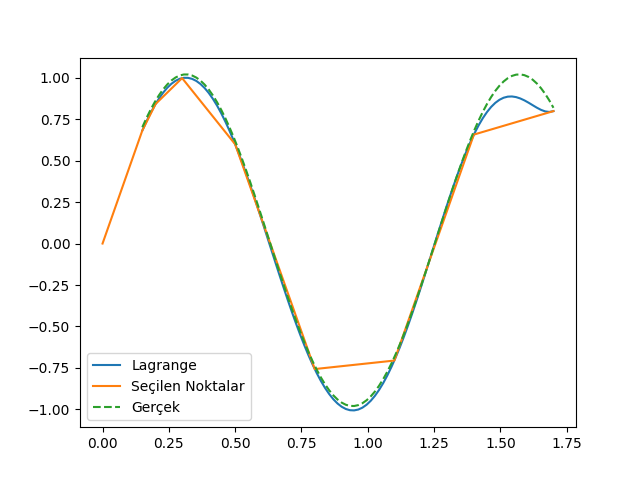
\includegraphics[width=20em]{compscieng_app20cfit1_01.png}

Kaynaklar

[1] Beu, {\em Introduction to Numerical Programming A Practical Guide for Scientists and Engineers Using Python and C/C++}

\end{document}




